% ============================================================
% 第 13 章 广义（上）同调理论
% 底本：原书 p.189–p.202 顶部（(13.98) 之后为 References，不属本章）
% 原文无编号定义/定理环境，只有节与编号公式
% ============================================================

\chapter{广义（上）同调理论}

% [原文 p.189]
到此为止我们讨论了
\begin{itemize}
  \item $H^{d+1}(BG;U(1))$，它描述 $d+1$ 维玻色子可逆相的 Dijkgraaf--Witten 相；
  \item $K^{d-i}(\pt)$ 与 $KO^{d-i}(\pt)$，它们描述 $d$ 维中具有各种对称型 $i$ 的自由费米子可逆相；
  \item $(I_{\Z}\Omega^{\mathcal S})^{d+2}(BG)$，它描述具有时空结构 $\mathcal S$ 的相对论性相互作用可逆相。
\end{itemize}
它们都是广义上同调理论的例子。事实上 Kitaev [Kit15] 有一个论证（后来由 Gaiotto 与 Johnson-Freyd [GJF17] 补充完善）：任何关于可逆相的分类结果都应当给出一个广义上同调理论。这促使我们从数学的观点来研究这个课题。

\section{公理}

我们考虑过（上）同调的多种定义：单纯（上）同调、胞腔（上）同调、$\R$ 系数的 de Rham 上同调等等。对性质良好的空间 $X$，它们全都一致。Eilenberg 与 Steenrod 把这种一致性公理化如下。

考虑为空间 $X$ 指定 Abel 群 $E^d(X)$，使得
\begin{enumerate}
  \item 对任意 $f:X\to Y$，有拉回 $f^*:E^d(Y)\to E^d(X)$。
  \item $f^*$ 只依赖于映射 $f$ 的同伦类。
\end{enumerate}
现在，设 $(X,p)$ 是带基点的空间（这只是说我们选定了点 $p\in X$ 作为基点）。可以证明必然有直和分解
\begin{equation}
E^d(X)=E^d(\pt)\oplus\tilde E^d(X). \tag{13.1}
\end{equation}
注意 $E^d(\pt)=\tilde E^d(S^0)$。下面我们刻画 $\tilde E^d(X)$ 而不是 $E^d(X)$。
\begin{enumerate}
  \setcounter{enumi}{2}
  \item 对带基点空间的包含 $A\subset X$，考虑序列
\begin{equation}
A\to X\to X/A. \tag{13.2}
\end{equation}
则相伴的序列
\begin{equation}
\tilde E^d(X/A)\to\tilde E^d(X)\to\tilde E^d(A) \tag{13.3}
\end{equation}
正合。
  \item 对悬挂 $\Sigma X:=X\times[0,1]/((p\times[0,1])\cup X\times\{1\})$，有
\begin{equation}
\tilde E^d(X)=\tilde E^{d+1}(\Sigma X). \tag{13.4}
\end{equation}
\end{enumerate}

% [原文 p.190]
\begin{enumerate}
  \setcounter{enumi}{4}
  \item 有
\begin{equation}
\tilde E^d(S^0)=
\begin{cases}
A & (d=0),\\
0 & (d\neq0).
\end{cases} \tag{13.5}
\end{equation}
\end{enumerate}
Eilenberg 与 Steenrod 证明了任何这样的指定必然彼此一致。现在，上面列出的各种上同调定义都可以证明满足这组公理，因此被迫全部相等。

广义上同调理论是把最后一条公理 (5)（称为维数公理）减弱而得到的：允许 $E^d(\pt)=\tilde E^d(S^0)$ 是任意的 Abel 群序列。例如，
\begin{itemize}
  \item 对 $K$ 理论，有
\begin{equation}
K^i(\pt)=
\begin{cases}
\Z & (i\ \text{为偶数}),\\
0 & (i\ \text{为奇数}),
\end{cases} \tag{13.6}
\end{equation}
  \item 对 $KO$ 理论，有
\begin{equation}
\begin{array}{c|cccccccc}
i\bmod 8 & 0 & -1 & -2 & -3 & -4 & -5 & -6 & -7\\ \hline
KO^i(\pt) & \Z & \Z_2 & \Z_2 & 0 & \Z & 0 & 0 & 0
\end{array} \tag{13.7}
\end{equation}
\end{itemize}
注意 $K^d(X)$ 与 $KO^d(X)$ 分别关于 $d$ 是 2-周期与 8-周期的。特别地，它们在 $d$ 取正值与负值时都可能非零。

注意在现代数学中，加上或去掉前缀 co 时，箭头方向反转。于是普通同调理论与广义同调理论也可以用下面这组公理类似地刻画。考虑为空间 $X$ 指定 Abel 群 $E_d(X)$，我们假定
\begin{enumerate}
  \item 对任意 $f:X\to Y$，有 $f_*:E_d(Y)\to E_d(X)$。
  \item $f_*$ 只依赖于映射 $f$ 的同伦类。
\end{enumerate}
像前面一样，有
\begin{equation}
E_d(X)=E_d(\pt)\oplus\tilde E_d(X), \tag{13.8}
\end{equation}
其中 $E_d(\pt)=\tilde E_d(S^0)$。然后
\begin{enumerate}
  \setcounter{enumi}{2}
  \item 对带基点空间的包含 $A\subset X$，考虑序列
\begin{equation}
A\to X\to X/A. \tag{13.9}
\end{equation}
则相伴的序列
\begin{equation}
\tilde E_d(A)\to\tilde E_d(X)\to\tilde E_d(X/A) \tag{13.10}
\end{equation}
正合。
  \item 对悬挂 $\Sigma X:=X\times[0,1]/((p\times[0,1])\cup X\times\{1\})$，有
\begin{equation}
\tilde E_d(X)=\tilde E_{d+1}(\Sigma X). \tag{13.11}
\end{equation}
\end{enumerate}

% [原文 p.191]
\begin{enumerate}
  \setcounter{enumi}{4}
  \item 有
\begin{equation}
\tilde E_d(S^0)=
\begin{cases}
A & (d=0),\\
0 & (d\neq0).
\end{cases} \tag{13.12}
\end{equation}
\end{enumerate}
这组公理唯一刻画了普通同调 $H_d(X;A)$。去掉公理 (5) 并把它换成任意的 Abel 群序列，就得到广义同调理论。例如，具有 $\mathcal S$ 结构的流形的配边群 $\Omega_d^{\mathcal S}(X)$ 都是广义同调理论；它们最初几个 $d$ 的取值 $\Omega_d^{\mathcal S}(\pt)$ 见表 10。

\takeaway{本节把 Eilenberg--Steenrod 公理减弱：保留同伦不变性、正合性与悬挂同构，只放开维数公理，就让 $E^d(\pt)$ 可取任意 Abel 群序列；$K$、$KO$ 与配边理论都是这样的广义（上）同调理论。}

\section{分类空间与 $\Omega$ 谱}

任何一个广义上同调理论 $E^d(X)$ 都有一列分类空间，使得
\begin{equation}
E^d(X)=[X,\mathcal E_d]. \tag{13.13}
\end{equation}
这些空间 $\mathcal E_d$ 可以选得满足
\begin{equation}
\mathcal E_d\simeq\Omega\mathcal E_{d+1}, \tag{13.14}
\end{equation}
其中 $\Omega X$ 表示 $X$ 的带基点环路空间。满足此条件的一列空间 $\{\mathcal E_d\}$ 称为 $\Omega$ 谱。

Kitaev 关于可逆相（带有你选定的各种条件，例如相对论性/非相对论性、自由/相互作用）应当由某个广义上同调理论给出的想法，来自他对可逆相分类空间的思考。固定要施加的条件集合，令 $\mathcal H_d$ 为 $d$ 维空间中满足这些条件的允许的“局部可逆有能隙哈密顿量”的集合。然后他考虑两个操作
\begin{equation}
\Omega\mathcal H_{d+1}\to\mathcal H_d \tag{13.15}
\end{equation}
与
\begin{equation}
\mathcal H_d\to\Omega\mathcal H_{d+1}. \tag{13.16}
\end{equation}
第一个操作 (13.15) 是把薄板上的、带有空间变化的 $(d+1)$ 维可逆系统看成单个 $d$ 维可逆有能隙系统。第二个操作 (13.16) 是把 $d$ 维可逆有能隙系统插入平凡的 $(d+1)$ 维薄板再把它抹平。然后需要论证这两个操作 (13.15) 与式 (13.16) 在差一个同伦的意义下互逆。这是一个有许多漏洞但颇为可信的论证，它为此后的许多进展提供了大量动机。此外，还有若干尝试想把这个论证严格化。

回到数学上来。任何一个广义同调理论 $E_d(X)$ 都可以用 $\Omega$ 谱 $\mathcal E_d$ 通过
\begin{equation}
E_d(X)=\lim_{n\to\infty}\pi_n(X\wedge\mathcal E_{n-d}) \tag{13.17}
\end{equation}
给出。

% [原文 p.192]
我们注意到下面的关系：
\begin{equation}
\pi_0(\mathcal E_d)=E^d(\pt)=E_{-d}(\pt). \tag{13.18}
\end{equation}
例如，$H^d(X;A)$ 与 $H_d(X;A)$ 的 $\Omega$ 谱由 $\{K(A,d)\}$ 给出，其中 $K(A,d)$ 是 Eilenberg--MacLane 空间。类似地，$K^d(X)$ 与 $KO^d(X)$ 的 $\Omega$ 谱分别由
\begin{equation}
\begin{array}{c|cc}
i\bmod 2 & 0 & -1\\ \hline
K_i & BU\times\Z & U
\end{array} \tag{13.19}
\end{equation}
与
\begin{equation}
\begin{array}{c|cccccccc}
i\bmod 8 & 0 & -1 & -2 & -3 & -4 & -5 & -6 & -7\\ \hline
KO_i & BO\times\Z & O & O/U & U/Sp & BSp\times\Z & Sp & Sp/U & U/O
\end{array} \tag{13.20}
\end{equation}
给出，见式 (11.41) 与式 (11.42)。这些分类空间通过式 (13.17) 定义了 $K$-同调 $K_i(X)$ 与 $KO$-同调 $KO_i(X)$。

配边群 $\Omega_d^{\mathcal S}(X)$ 的谱称为 Thom 谱，通常记作 $M\mathcal S_d$。这个谱定义了相应的广义上同调群，通常称为配边上同调，但有时也简称配边群，记作 $\Omega_{\mathcal S}^d(X)$。它在几何上定义为
\begin{equation}
\Omega_{\mathcal S}^d(X):=\frac{\{\text{余维为 }d\text{ 的 proper 映射 }Z\to X\}}{\text{配边}}, \tag{13.21}
\end{equation}
其中映射应当在余维方向上具有 $\mathcal S$ 结构。

\takeaway{每个广义上同调理论都由一列分类空间 $\mathcal E_d$ 表示，$E^d(X)=[X,\mathcal E_d]$；条件 $\mathcal E_d\simeq\Omega\mathcal E_{d+1}$ 即 $\Omega$ 谱。Kitaev 借可逆相分类空间的两个互逆操作，论证相的分类必是广义上同调理论。}

\section{Anderson 对偶}

然而还有另一种办法，可以从广义同调理论得到广义上同调理论。为此回忆普通（上）同调的万有系数定理：
\begin{equation}
0\to\operatorname{Ext}(H_{p-1}(M;\Z),\Z)\to H^p(M;\Z)\to\operatorname{Hom}(H_p(M;\Z),\Z)\to0, \tag{13.22}
\end{equation}
其中
\begin{equation}
\operatorname{Ext}(A,\Z)=\operatorname{Hom}(A\text{ 的挠部分},\R/\Z). \tag{13.23}
\end{equation}
对广义（上）同调理论 $E_d$ 与 $E^d$，下面这个序列不成立：
\begin{equation}
0\to\operatorname{Ext}(E_{p-1}(M),\Z)\to E^p(M)\to\operatorname{Hom}(E_p(M),\Z)\to0. \tag{13.24}
\end{equation}
但已知存在另一个广义（上）同调理论 $(I_{\Z}E)_d$ 与 $(I_{\Z}E)^d$，使得下面这个序列成立：
\begin{equation}
0\to\operatorname{Ext}(E_{p-1}(M),\Z)\to(I_{\Z}E)^p(M)\to\operatorname{Hom}(E_p(M),\Z)\to0. \tag{13.25}
\end{equation}
$(I_{\Z}E)^d(X)$ 称为 $E_d(X)$ 的 Anderson 对偶。

% [原文 p.193]
于是普通（上）同调的万有系数定理意味着：对 $h^d(X):=H^d(X;\Z)$，有
\begin{equation}
(I_{\Z}h)^d(X)=h^d(X). \tag{13.26}
\end{equation}
类似地，已知
\begin{equation}
(I_{\Z}K)^d(X)=K^d(X) \tag{13.27}
\end{equation}
而
\begin{equation}
(I_{\Z}KO)^d(X)=KO^{d-4}(X). \tag{13.28}
\end{equation}
上面我们看到，$d+1$ 维中带 spin 结构的相互作用费米子可逆相由 $(I_{\Z}\Omega^{\mathrm{spin}})^{d+2}(X)$ 分类。相应的自由相属于 D 型，由 $KO^{d-2}(X)$ 分类。于是存在自然的从自由到相互作用的映射
\begin{equation}
KO^{d-2}(X)\to(I_{\Z}\Omega^{\mathrm{spin}})^{d+2}(X). \tag{13.29}
\end{equation}
对这个映射的数学理解如下。在指标定理的语境中，Atiyah、Bott 与 Shapiro 找到了一种把 spin $d$-流形变成 $KO$-同调中一个类的办法：
\begin{equation}
\Omega_d^{\mathrm{spin}}(\pt)\to KO_d(\pt). \tag{13.30}
\end{equation}
这可以做成族版本：
\begin{equation}
\Omega_d^{\mathrm{spin}}(X)\to KO_d(X). \tag{13.31}
\end{equation}
现在我们取两边的 Anderson 对偶：
\begin{equation}
(I_{\Z}KO)^d(X)\to(I_{\Z}\Omega^{\mathrm{spin}})^d(X), \tag{13.32}
\end{equation}
这里箭头反转是因为我们取了对偶。利用式 (13.28)，得到
\begin{equation}
KO^{d-4}(X)\to(I_{\Z}\Omega^{\mathrm{spin}})^d(X), \tag{13.33}
\end{equation}
这正是我们上面讨论过的从自由到相互作用的同态。

类似地，有自然映射
\begin{equation}
\Omega_d^{\mathcal S}(X)\to H_d(X;\Z), \tag{13.34}
\end{equation}
它把配边类 $[M_d,f:M_d\to X]$ 送到 $f(M_d)\subset X$ 的同调类。取 Anderson 对偶并利用 $H^d(-;\Z)$ 的 Anderson 自对偶性，我们有
\begin{equation}
H^d(X;\Z)\to(I_{\Z}\Omega^{\mathcal S})^d(X). \tag{13.35}
\end{equation}
这把 Dijkgraaf--Witten 相重新解释为具有 $\mathcal S$ 时空结构的相互作用可逆相。

一般来说，最后这个映射既不是满射也不是单射，即使 $\mathcal S$ 取定向也是如此。对偶地，映射 (13.34) 也不一定满射或单射。作为本系列讲座的最后一个课题，我们来讨论这些问题。

\takeaway{Anderson 对偶 $(I_{\Z}E)^d$ 使万有系数短正合列对广义理论也成立；$KO$ 的对偶是 $KO^{d-4}$。由此得到自由费米子相到相互作用相的自然映射，以及 Dijkgraaf--Witten 相到配边上同调的映射。}

\section{Atiyah--Hirzebruch--Leray--Serre 谱序列}

% [原文 p.194]
首先我们需要知道一些计算 $\Omega_d^{\mathcal S}(X)$ 的方法，更一般地，计算广义（上）同调理论 $T$ 的 $T_d(X)$ 或 $T^d(X)$ 的方法。基本工具是 Atiyah--Hirzebruch--Leray--Serre 谱序列。

考虑纤维化 $F\to X\to B$。AHLS 谱序列使我们能由 $H_*(X;\Z)$ 与 $T_*(F)$ 的知识“确定” $T_*(X)$；或者对偶地，由 $H^*(X;\Z)$ 与 $T^*(F)$ 的知识“确定” $T^*(X)$。引号的原因很快就会解释。

当 $T=H$ 时，这套机制可用来由纤维 $F$ 与底空间 $B$ 的（上）同调群的数据确定全空间 $X$ 的（上）同调。当 $T\neq H$ 时，这套机制通常通过把它应用于 $\pt\to X\to X$ 来使用，使我们能由 $H_*(X;\Z)$ 与 $T_*(\pt)$ 等（在一定程度上）确定 $T_*(X)$。

\subsection{同调的谱序列}

先对 $T_*(X)$ 来描述。回忆 $B$ 有一列骨架 $B_0\subset B_1\subset B_2\subset\cdots$，其中 $B_k$ 包含维数至多为 $k$ 的胞腔。考虑 $X$ 的递增子集 $f^{-1}(B_0)\subset f^{-1}(B_1)\subset\cdots$，其中 $f:X\to B$ 是投影。定义
\begin{equation}
G_{k,d-k}:=\operatorname{Im}\iota_*:T_d(f^{-1}(B_k))\to T_d(X). \tag{13.36}
\end{equation}
这构成滤过
\begin{equation}
G_{0,d}\subset G_{1,d-1}\subset G_{2,d-2}\subset\cdots\subset G_{d,0}=T_d(X). \tag{13.37}
\end{equation}
然后可以取“相伴分次”
\begin{equation}
\operatorname{Gr}(T_d(X)):=G_{0,d}\oplus\frac{G_{1,d-1}}{G_{0,d}}\oplus\frac{G_{2,d-2}}{G_{1,d-1}}\oplus\cdots\oplus\frac{G_{d,0}}{G_{d-1,1}}. \tag{13.38}
\end{equation}
知道式 (13.38) 并不能唯一确定 $T_d(X)$，但会极大地约束它。谱序列所“计算”的正是式 (13.38)。（引号的原因同样很快就会解释。）

具体做法如下。先构造所谓 $E_2$ 页：
\begin{equation}
E_{p,q}^2=H_p(B;E_q(F)). \tag{13.39}
\end{equation}
它有形式为
\begin{equation}
d^2:E_{p,q}^2\to E_{p-2,q+1}^2 \tag{13.40}
\end{equation}
的微分，满足 $d^2\circ d^2=0$。

这里的上标 $2$ 并不是取平方的意思，它只是说这是第二页上的一个微分。微分把 $p+q=n$ 连到 $p+q=n-1$。习惯上把 $p$

% [原文 p.195]
画成水平方向、$q$ 画成竖直方向。于是 $d^2$ 向上走一步、向左走两步：
% [图：原书 p.195，按原图裁切，未重绘]
\begin{equation}
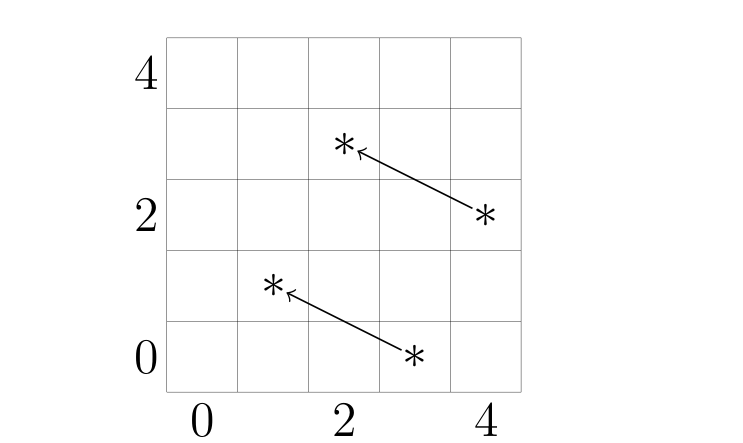
\includegraphics[width=0.40\textwidth]{figures/fig13_41.png} \tag{13.41}
\end{equation}
然后取它的上同调来定义 $E^3$ 页：
\begin{equation}
E_{p,q}^3=\frac{\operatorname{Ker}\left(d^2:E_{p,q}^2\to E_{p-2,q+1}^2\right)}
{\operatorname{Im}\left(d^2:E_{p+2,q-1}^2\to E_{p,q}^2\right)}, \tag{13.42}
\end{equation}
已知它有形式为
\begin{equation}
d^3:E_{p,q}^3\to E_{p-3,q+2}^3 \tag{13.43}
\end{equation}
的微分，满足 $d^3\circ d^3=0$。$E^4$ 页类似地定义为
\begin{equation}
E_{p,q}^4=\frac{\operatorname{Ker}\left(d^3:E_{p,q}^3\to E_{p-3,q+2}^3\right)}
{\operatorname{Im}\left(d^3:E_{p+3,q-2}^3\to E_{p,q}^3\right)}, \tag{13.44}
\end{equation}
它有形式为
\begin{equation}
d^4:E_{p,q}^4\to E_{p-4,q+3}^4 \tag{13.45}
\end{equation}
的微分，如此无限继续。最终得到 $E_{p,q}^\infty$，它通过
\begin{equation}
\operatorname{Gr}(T_d(X))=E_{0,d}^\infty\oplus E_{1,d-1}^\infty\oplus E_{2,d-2}^\infty\oplus\cdots\oplus E_{d,0}^\infty \tag{13.46}
\end{equation}
给出式 (13.38)。

整个结构常被缩写为
\begin{equation}
E_{p,q}^2=H_p(B;T_q(F))\Rightarrow T_{p+q}(X). \tag{13.47}
\end{equation}

\subsection{上同调的谱序列}

下面来对 $T^*(X)$ 描述它。此时滤过的方向相反：
\begin{equation}
T^d(X)=G^{0,d}\supset G^{1,d-1}\supset G^{2,d-2}\supset\cdots\supset G^{d,0}. \tag{13.48}
\end{equation}
然后可以取“相伴分次”
\begin{equation}
\operatorname{Gr}(T^d(X)):=\frac{G^{0,d}}{G^{1,d-1}}\oplus\frac{G^{1,d-1}}{G^{2,d-2}}\oplus\cdots\oplus G^{d,0}. \tag{13.49}
\end{equation}

% [原文 p.196]
$E_2$ 页现在是
\begin{equation}
E_2^{p,q}=H^p(B;E^q(F)). \tag{13.50}
\end{equation}
它有形式为
\begin{equation}
d_2:E_2^{p,q}\to E_2^{p+2,q-1} \tag{13.51}
\end{equation}
的微分，满足 $d_2\circ d_2=0$。$E^3$ 页是它的上同调：
\begin{equation}
E_3^{p,q}=\frac{\operatorname{Ker}\left(d_2:E_2^{p,q}\to E_2^{p+2,q-1}\right)}
{\operatorname{Im}\left(d_2:E_2^{p-2,q+1}\to E_2^{p,q}\right)}, \tag{13.52}
\end{equation}
它有
\begin{equation}
d_3:E_3^{p,q}\to E_3^{p+3,q-2} \tag{13.53}
\end{equation}
满足 $d^3\circ d^3=0$。$E^4$ 页则是
\begin{equation}
E_4^{p,q}=\frac{\operatorname{Ker}\left(d_3:E_3^{p,q}\to E_3^{p+3,q-2}\right)}
{\operatorname{Im}\left(d_3:E_3^{p-3,q+2}\to E_3^{p,q}\right)}, \tag{13.54}
\end{equation}
它有形式为
\begin{equation}
d_4:E_4^{p,q}\to E_4^{p+4,q-3} \tag{13.55}
\end{equation}
的微分，如此无限继续。最终得到 $E_\infty^{p,q}$，它通过
\begin{equation}
\operatorname{Gr}(T^d(X))=E_\infty^{0,d}\oplus E_\infty^{1,d-1}\oplus E_\infty^{2,d-2}\oplus\cdots\oplus E_\infty^{d,0} \tag{13.56}
\end{equation}
给出式 (13.49)。整个结构常被缩写为
\begin{equation}
E_2^{p,q}=H^p(B;T^q(F))\Rightarrow T^{p+q}(X). \tag{13.57}
\end{equation}

\takeaway{AHLS 谱序列由纤维化 $F\to X\to B$ 计算 $T_*(X)$：$E^2_{p,q}=H_p(B;T_q(F))$，微分 $d^r$ 的双次数为 $(-r,r-1)$，其极限 $E^\infty$ 给出滤过的相伴分次 $\operatorname{Gr}(T_d(X))$，再经扩张问题回推 $T_d(X)$。}

\section{配边群的一些计算}

\subsection{自旋配边}

让我们试着从这套庞大的机器中获得一些经验。首先用 $\Omega_d^{\mathrm{spin}}(X)$。取纤维化 $\pt\to X\to X$ 并使用 AHLS 谱序列，它具有形式
\begin{equation}
E_{p,q}^2=H_p(X;\Omega_q^{\mathrm{spin}}(\pt))\Rightarrow\Omega_{p+q}^{\mathrm{spin}}(X). \tag{13.58}
\end{equation}
我们知道 $\Omega_{0,1,2,3,4}^{\mathrm{spin}}(\pt)=\Z,\Z_2,\Z_2,0,\Z$。取 $X=B\Z_2=\R\mathrm{P}^\infty$，对此我们知道
\begin{equation}
H_{0,1,2,3,4,\ldots}(B\Z_2;\Z)=\Z,\Z_2,0,\Z_2,0,\Z_2,\ldots \tag{13.59}
\end{equation}
\begin{equation}
H_{0,1,2,3,4,\ldots}(B\Z_2;\Z_2)=\Z_2,\Z_2,\Z_2,\Z_2,\Z_2,\ldots \tag{13.60}
\end{equation}

% [原文 p.197]
于是 $E^2$ 页具有如下形式：
% [图：原书 p.197，按原图裁切，未重绘]
\begin{equation}
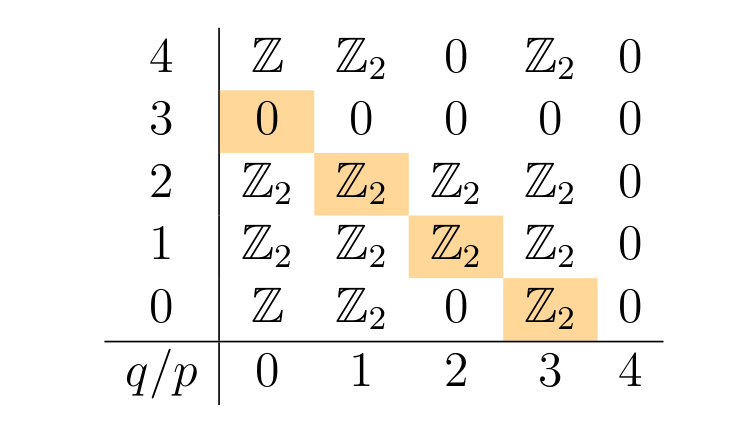
\includegraphics[width=0.34\textwidth]{figures/fig13_61.png} \tag{13.61}
\end{equation}
由 $E^2$ 得到 $E^3$、由 $E^3$ 得到 $E^4$ 都需要取上同调。因此这会使各项“变小”。另外，$\operatorname{Gr}(T_k(X))$ 是有限群，$|\operatorname{Gr}(T_k(X))|=|T_k(X)|$。由此，从上方的 $E^2$ 页容易推出
\begin{equation}
|\Omega_3^{\mathrm{spin}}(B\Z_2)|\leq 8. \tag{13.62}
\end{equation}
由 eta 不变量的计算，我们还知道
\begin{equation}
\eta(S^3/\Z_2,\text{非平凡 }\Z_2\text{ 丛})=1/8 \tag{13.63}
\end{equation}
因此 $[S^3/\Z_2,\text{非平凡 }\Z_2\text{ 丛}]\subset\Omega_3^{\mathrm{spin}}(B\Z_2)$ 生成一个 $\Z_{8k}$ 子群。结合起来，我们断定
\begin{equation}
\Omega_3^{\mathrm{spin}}(B\Z_2)=\Z_8. \tag{13.64}
\end{equation}
这也表明对 $p+q=3$ 有 $E_{p,q}^2=E_{p,q}^\infty$，并且滤过为
\begin{equation}
0\subset\Z_2\subset\Z_4\subset\Z_8=\Omega_3^{\mathrm{spin}}(B\Z_2) \tag{13.65}
\end{equation}
其相伴分次由
\begin{equation}
0\subset\Z_2\oplus\frac{\Z_4}{\Z_2}\oplus\frac{\Z_8}{\Z_4} \tag{13.66}
\end{equation}
给出。

\subsection{定向配边}

接下来考虑 $\Omega_n^{\mathrm{oriented}}(X)$。取纤维化 $\pt\to X\to X$ 并使用 AHLS 谱序列，它具有形式
\begin{equation}
E_{p,q}^2=H_p(X;\Omega_q^{\mathrm{oriented}}(\pt))\Rightarrow\Omega_{p+q}^{\mathrm{oriented}}(X). \tag{13.67}
\end{equation}
由于 $\Omega_{0,1,2,3,4,5}^{\mathrm{oriented}}(\pt)=\Z,0,0,0,\Z,\Z_2$，$E^2$ 页具有如下形式：
% [图：原书 p.197，按原图裁切，未重绘]
\begin{equation}
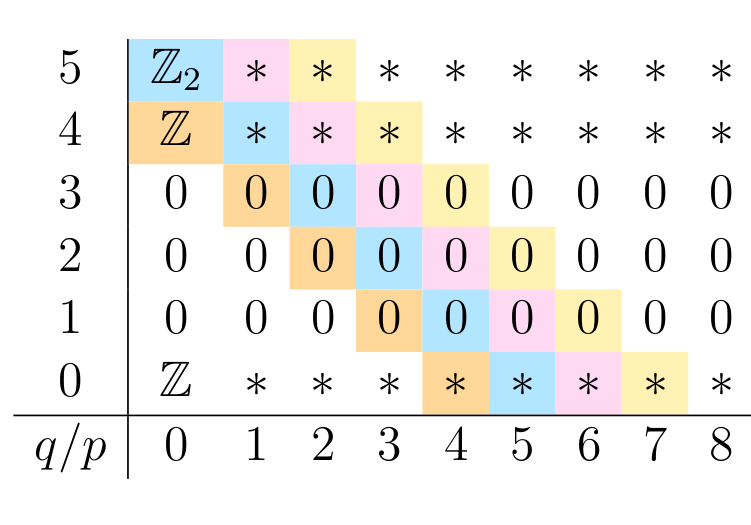
\includegraphics[width=0.36\textwidth]{figures/fig13_68.png} \tag{13.68}
\end{equation}

% [原文 p.198]
由此我们容易断定
\begin{equation}
\Omega_n^{\mathrm{oriented}}(X)=H_n(X;\Z),\qquad n=0,1,2,3. \tag{13.69}
\end{equation}
另外回忆一般有
\begin{equation}
E_n(X)=E_n(\pt)\oplus\tilde E_n(X) \tag{13.70}
\end{equation}
这意味着 $E^2$ 页的第零列需要一直存活到 $E^\infty$，也就是说，任何进入第零列的 $d^k$ 都是零映射。此外，它不会进入由 $E_{p,q}^\infty$ 恢复 $\Omega_n^{\mathrm{oriented}}(X)$ 的扩张问题。这使我们容易地确定 $n=4$ 的情形为
\begin{equation}
\Omega_4^{\mathrm{oriented}}(X)=\Omega_4^{\mathrm{oriented}}(\pt)\oplus\tilde\Omega_4^{\mathrm{oriented}}(X)=\Z\oplus H_4(X;\Z). \tag{13.71}
\end{equation}
$n=5$ 的情形较难确定，但由 $E_{5,0}^5=H_5(X;\Z)$ 出发的 $d^5$ 是零，因为它到达 $E_{0,4}^5=\Omega_4^{\mathrm{oriented}}(X)$，正如我们上面论证的那样。现在需要考虑微分
\begin{equation}
d^5:(E_{6,0}^5)=H_6(X;\Z)\to(E_{1,4}^5)=H_1(X;\Z), \tag{13.72}
\end{equation}
但已知这个映射一般是零（详见下文）。这使我们能计算 $E^6$ 页，而 $d^6$ 及以后的微分都因次数原因而为零。我们断定：
\begin{equation}
\Omega_5^{\mathrm{oriented}}(X)=\Omega_5^{\mathrm{oriented}}(\pt)_{=\Z_2}\oplus\tilde\Omega_5^{\mathrm{oriented}}(X), \tag{13.73}
\end{equation}
其中有短正合列
\begin{equation}
0\to H_1(X;\Z)\to\tilde\Omega_5^{\mathrm{oriented}}(X)\to H_5(X;\Z)\to0. \tag{13.74}
\end{equation}
特别地，$H_5(X;\Z)$ 中任何同调类都可以实现为映射 $f:M_5\to X$ 的像 $f(M_5)$，其中 $M_5$ 是流形。

$n=6$ 的情形更难，但式 (13.72) 的消失保证了 $E_{6,0}^5$ 存活到 $E_{6,0}^\infty$，这意味着
\begin{equation}
\tilde\Omega_6^{\mathrm{oriented}}(X)\to H_6(X;\Z) \tag{13.75}
\end{equation}
是满射。这意味着任何 6 次同调类都是某个流形的像 $f(M_6)$，即 $f:M_6\to X$。

$n=7$ 的情形更有趣，因为微分
\begin{equation}
d^5:(E_{7,0}^5)=H_7(X;\Z)\to(E_{2,4}^5)=H_2(X;\Z) \tag{13.76}
\end{equation}
实际上可以非平凡：
% [图：原书 p.198，按原图裁切，未重绘]
\begin{equation}
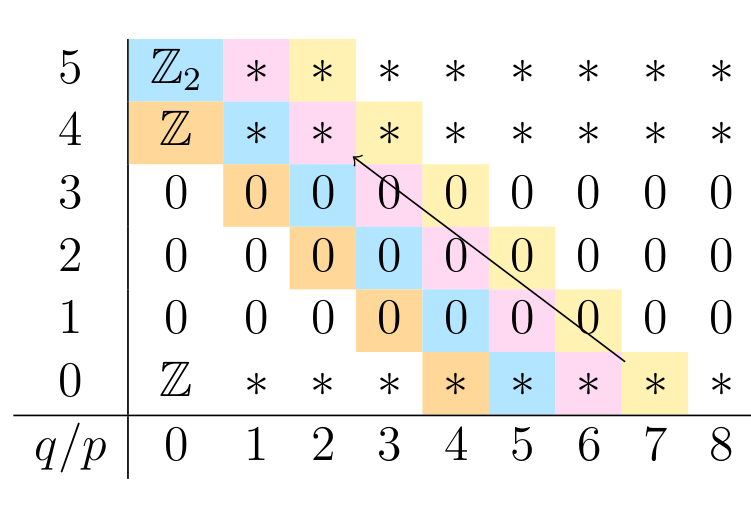
\includegraphics[width=0.36\textwidth]{figures/fig13_77.png} \tag{13.77}
\end{equation}

% [原文 p.199]
这意味着
\begin{equation}
E_{7,0}^6=\operatorname{Ker}\left(d^5:E_{7,0}^5\to E_{2,4}^5\right)\subset H_7(X;\Z) \tag{13.78}
\end{equation}
可以是真子集，也就是说映射
\begin{equation}
\tilde\Omega_7^{\mathrm{oriented}}(X)\to H_7(X;\Z) \tag{13.79}
\end{equation}
的像（它等于 $E_{7,0}^6\simeq E_{7,0}^\infty$）是 $H_7(X;\Z)$ 的真子集。这引出一个惊人的结论：并非 $H_7(X;\Z)$ 的所有元素都能实现为映射 $f:M_7\to X$ 的像 $f(M_7)$，更不用说由嵌入子流形 $\iota:M_7\subset X$ 实现。

一个非常好的显式例子在 [BHK00] 的 arXiv 第 1 版中讨论过\footnote[22]{发表版对应 arXiv 上的第 2 版，那里讨论的是 $H_7(X;\Z)$ 中一个更微妙的类：它不能由嵌入子流形实现，但可以由某个流形的像实现。这个例子出奇地简单。取 $X=Sp(2)$，即维数为 10 的辛群 $Sp(2)$ 的群流形。它非零的整同调群为 $H_{0,3,7,10}(Sp(2);\Z)$，全都是 $\Z$。$\Z\cong H_3(Sp(2);\Z)$ 的生成元由子群 $S^3\cong SU(2)\cong Sp(1)\subset Sp(2)$ 实现，这显然是子流形。但 $\Z\cong H_7(Sp(2);\Z)$ 的生成元不能这样实现；只有 $3\in\Z$ 才有子流形代表。}。为此他们取 $X=S^7/\Z_3\times S^3/\Z_3$。设 $v_{1,2}$ 是 $H^1(S^{3,7}/\Z_3;\Z_3)\cong\Z_3$ 的生成元。考虑元素 $x:=\ol{\beta}(v_1v_2)\in H^3(X;\Z)$，其中
\begin{equation}
\ol{\beta}:H^d(X;\Z_3)\to H^{d+1}(X;\Z) \tag{13.80}
\end{equation}
是 Bockstein。那么 $x$ 的 Poincaré 对偶 $y\in H_7(X;\Z)$ 不在 $d^4$ 的核中，因而不能实现为从流形出发的映射的像。

映射
\begin{equation}
\Omega_d^{\mathrm{oriented}}(X)\to H_d(X;\Z) \tag{13.81}
\end{equation}
的非满性导致
\begin{equation}
H^d(X;\Z)\to(I_{\Z}\Omega^{\mathrm{oriented}})^d(X;\Z) \tag{13.82}
\end{equation}
的非单性。

这意味着某些 Dijkgraaf--Witten 相只要在流形上求值就实际是平凡的（但在三角剖分的多面体上求值时可以非平凡）。第一个这样的例子是 $(6+1)$ 维 Dijkgraaf--Witten 可逆相。

例如取对称性 $\Z_3\times\Z_3$。回忆 $H^1(B\Z_3;\Z_3)=\Z_3$，其生成元 $A$ 就是 $\Z_3$ 规范场。$H^2(B\Z_3;\Z_3)=\Z_3$ 由其 Bockstein $\beta A$ 生成。现在对 $\Z_3\times\Z_3$ 取它的两份拷贝。$6+1$ 维中任意的 Dijkgraaf--Witten 作用就是从 $(\beta A_1)^n(\beta A_2)^m$ 中剥离出一个 $\beta$，其中 $n+m=4$。（若把 $\Z_3\subset U(1)$ 看待，它们实际上是 Abel Chern--Simons 项，其中 $\beta A_i\sim F_i$。）

现在考虑作用量
\begin{equation}
\mathcal P^1\beta(A_1\cup A_2)=(\beta A_1)^3A_2-A_1(\beta A_2)^3. \tag{13.83}
\end{equation}
在 7-流形 $M_7$ 上求值时，我们有公式
\begin{equation}
\int_{M_7}\mathcal P^1x_3=\int_{M_7}p_1(M_7)x_3 \tag{13.84}
\end{equation}

% [原文 p.200]
对一般的 $x_3\in H^3(M_7;\Z_3)$ 成立。把它应用于上面的情形，得到
\begin{equation}
\int_{M_7}\mathcal P^1\beta(A_1\cup A_2)=\int_{M_7}p_1(M_7)\beta(A_1\cup A_2). \tag{13.85}
\end{equation}
在定向流形上，$\beta$ 可以部分积分，于是
\begin{equation}
=-\int_{M_7}(\beta p_1(M_7))(A_1\cup A_2), \tag{13.86}
\end{equation}
但 $p_1(M_7)$ 是整系数类，所以它的 Bockstein 为零：
\begin{equation}
=-\int_{M_7}0\cdot A_1\cup A_2=0. \tag{13.87}
\end{equation}
这个上同调运算 $\mathcal P^1\beta$ 本质上是 $d^5:H_n(X;\Z)\to H_{n-5}(X;\Z)$ 的对偶，后者是 $d_5:H^{n-5}(X;\R/\Z)\to H^n(X;\R/\Z)$，由
\begin{equation}
d_5=\iota_{\Z_3\to\R/\Z}\mathcal P^1\beta_{\R/\Z\to\Z_3} \tag{13.88}
\end{equation}
给出，其中 $\iota$ 是改变系数群给出的同态，$\beta$ 是与 $0\to\R/\Z\xrightarrow{3\times}\R/\Z\to\Z_3\to0$ 相伴的 Bockstein。这意味着，按构造，类 $\mathcal P^1\beta(A_1\cup A_2)$ 在 Poincaré 对偶的同调圈 $y\in H_7(X;\Z)$ 上有非平凡的积分，而 $y$ 不是流形！

\takeaway{本节示范如何用 AHLS 谱序列算配边群：取 $X=B\Z_2$、$B\Z_3$ 等分类空间，$E^2_{p,q}=H_p(X;\Omega_q^{\mathrm{spin/\mathrm{SO}}}(\pt))$ 只涉及已知的同调群与低维配边群，微分 $d^5$ 由上同调运算 $\mathcal P^1\beta$ 给出，最终得到带 $B\Z_2$、$B\Z_3$ 系数的配边群。}

\section{$\pi_4(S^3)$}

上面我们用同调谱序列计算了 $\Omega_d^{\mathcal S}(X)$。上同调谱序列往往更易于处理，因为 $E_2$ 页 $E_2^{p,q}=H^p(B;T^q(F))$ 是一个分次代数（当 $T^q$ 具有乘法结构时），而 $d_2$ 是这个代数的导子；对更高的 $E^n$ 与 $d_n$ 也类似。

作为谱序列的最后一个应用，也为了看清分次代数结构的用处，我们来讨论经典的 $\pi_4(S^3)=\Z_2$ 计算：用 Leray--Serre 谱序列，这在任何代数拓扑基础教材中都能找到。下面的内容取自 [ST24, 附录 B]。首先需要把 $\pi_4(S^3)$ 的计算转化为某个上同调群的计算。这可以用下面的技巧做到。

考虑 $H^3(S^3;\Z)\cong\Z$ 的生成元的分类映射 $f:S^3\to K(\Z,3)$，令 $P$ 为其同伦纤维：
\begin{equation}
P\to S^3\to K(\Z,3). \tag{13.89}
\end{equation}
相应地，我们有如下形式的纤维化
\begin{equation}
K(\Z,2)\to P\to S^3. \tag{13.90}
\end{equation}

% [原文 p.201]
与式 (13.90) 相伴的同伦长正合列为
% [Tutor Note: 原文此处引作 (13.87)，按上下文应为 (13.90)，已登记进原文笔误表。]
\begin{equation}
\begin{array}{cccccc}
 & & \to & \pi_5(K(\Z,3))=0 & &\\
\to & \pi_4(P) & \to & \pi_4(S^3)=? & \to & \pi_4(K(\Z,3))=0\\
\to & \pi_3(P) & \to & \pi_3(S^3)=\Z & \xrightarrow{\sim} & \pi_3(K(\Z,3))=\Z\\
\to & \pi_2(P) & \to & \pi_2(S^3)=0 & \to & \pi_2(K(\Z,3))=0\\
\to & \pi_1(P) & \to & \pi_1(S^3)=0 & \to & \pi_1(K(\Z,3))=0\\
\to & \pi_0(P) & \to & \pi_0(S^3)=0 & \to & \pi_0(K(\Z,3))=0
\end{array} \tag{13.91}
\end{equation}
其中 $\pi_3(S^3)\cong\pi_3(K(\Z,3))$ 是由构造保证的。由此我们知道
\begin{equation}
\pi_{0,1,2,3}(P)=0,\qquad \pi_4(P)\cong\pi_4(S^3), \tag{13.92}
\end{equation}
而应用 Hurewicz 定理给出
\begin{equation}
H_0(P;\Z)=\Z,\quad H_{1,2,3}(P;\Z)=0,\quad H_4(P;\Z)\cong\pi_4(P)\cong\pi_4(S^3). \tag{13.93}
\end{equation}
因此只需计算 $H_4(P;\Z)$。

为此我们使用与 $K(\Z,2)\to P\to S^3$ 相伴的 $H^\bullet(P;\Z)$ 的 Leray--Serre 谱序列。回忆 $K(\Z,2)=\CP^\infty$，且 $H^*(K(\Z,2);\Z)=\Z[u]$，其中 $u$ 的次数为 2。设 $v$ 表示 $H^3(S^3;\Z)=\Z$ 的生成元。那么 $E_2$ 页就是
% [图：原书 p.201，按原图裁切，未重绘]
\begin{equation}
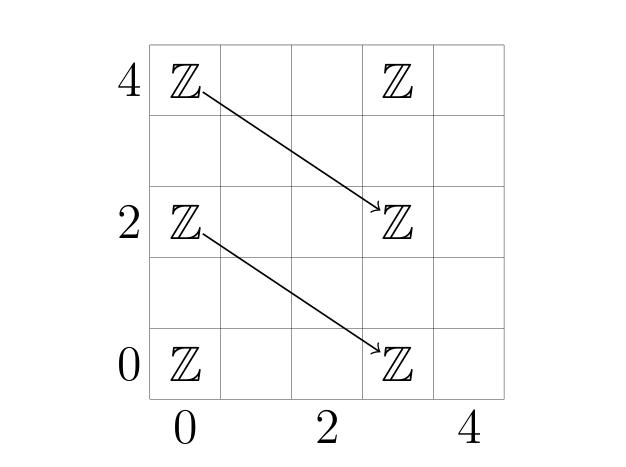
\includegraphics[width=0.34\textwidth]{figures/fig13_94.png} \tag{13.94}
\end{equation}
其中 $E_2^{0,2n}\cong\Z u^n$，$E_2^{3,2n}\cong\Z u^nv$。

由于 $E^2$ 页的稀疏性，$d_2$ 全是零映射。于是 $E^3=E^2$，我们需要考虑 $d_3$。为确定 $d_3$，注意由式 (13.91) 有 $H^2(P;\Z)=H^3(P;\Z)=0$。因此 $d_3:E_3^{0,2}\to E_3^{3,0}$ 应当是同构，由 $d_3u=v$ 给出。
% [Tutor Note: 原文此处作 $d_2u=v$，按上下文应为 $d_3u=v$，已登记进原文笔误表。]接着 $d_3:E_3^{0,4}\to E_3^{3,2}$ 是乘以 2，由 $d_3u^2=2uv$ 给出。因此 $E_4$ 页是
% [图：原书 p.201，按原图裁切，未重绘]
\begin{equation}
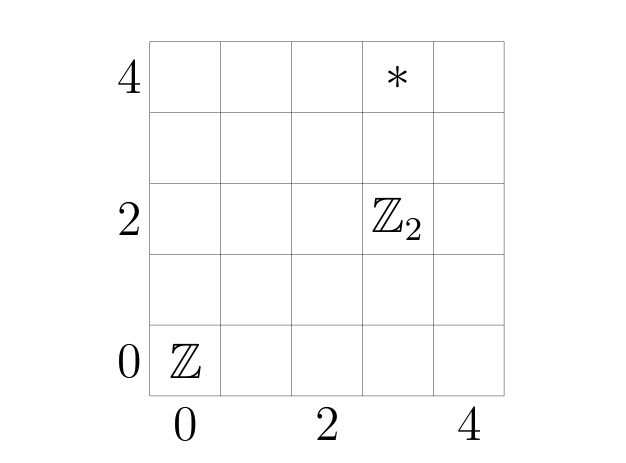
\includegraphics[width=0.34\textwidth]{figures/fig13_95.png} \tag{13.95}
\end{equation}
由此我们断定
\begin{equation}
H^4(P;\Z)=0,\qquad H^5(P;\Z)=\Z_2. \tag{13.96}
\end{equation}

% [原文 p.202]
因此我们有
\begin{equation}
H_4(P;\Z)=\Z_2, \tag{13.97}
\end{equation}
再由式 (13.91) 断定
\begin{equation}
\pi_4(S^3)=\Z_2. \tag{13.98}
\end{equation}

\takeaway{本节用 $K(\Z,2)\to P\to S^3$ 的 Leray--Serre 谱序列：$E_2^{0,2n}=\Z u^n$、$E_2^{3,2n}=\Z u^nv$，微分 $d_3u=v$、$d_3u^2=2uv$，得 $H^4(P)=0$、$H^5(P)=\Z_2$，从而 $\pi_4(S^3)=\Z_2$。}

\chapterreview{本章把可逆相的分类放进广义（上）同调理论的框架。§13.1 用 Eilenberg--Steenrod 公理说明普通（上）同调的唯一性，并指出放开维数公理即得广义理论。§13.2 引入分类空间与 $\Omega$ 谱，给出 $E^d(X)=[X,\mathcal E_d]$ 以及 Kitaev 的物理论证。§13.3 讨论 Anderson 对偶，得到自由相到相互作用相、Dijkgraaf--Witten 相到配边上同调的自然映射。§13.4 陈述 AHLS 谱序列的同调与上同调版本，并强调它只决定相伴分次对象。§13.5 用谱序列计算 自旋与定向配边群，借 $n=7$ 的非满性说明 $H_7$ 中并非所有类都能由流形实现。§13.6 以 Leray--Serre 谱序列算出 $\pi_4(S^3)=\Z_2$。}
